\documentclass[t]{beamer}
\usepackage{physics}
\usepackage{amsmath}
\usepackage{tikz}
\usepackage{mathdots}
\usepackage{yhmath}
\usepackage{cancel}
\usepackage{color}
\usepackage{siunitx}
\usepackage{array}
\usepackage{multirow}
\usepackage[version=4]{mhchem}
\usepackage{amssymb}
\usepackage{textcomp, gensymb}
\usepackage{mathtools}
\usepackage{pifont}
\newcommand{\cmark}{\ding{51}}%
\newcommand{\xmark}{\ding{55}}%
\usepackage{tabularx}
\usepackage{extarrows}
\usepackage{booktabs}
\usetikzlibrary{fadings}
\usetikzlibrary{patterns}
\usetikzlibrary{shadows.blur}
\usetikzlibrary{shapes}
\usepackage[style=verbose,backend=bibtex]{biblatex}
\addbibresource{wannier.bib}
\addbibresource{hubbard.bib}
\addbibresource{pt.bib}
\renewcommand{\footnotesize}{\scriptsize}
\usepackage{listings}
\usepackage{hyperref}

\newcommand{\pair}[1]{\langle #1 \rangle}
\DeclareMathOperator{\ee}{e}
\DeclareMathOperator{\ii}{i}
\DeclareMathOperator{\sgn}{sgn}

\newcommand{\concept}[1]{\textbf{#1}}
\newcommand*{\abinitio}{\textit{ab initio}}
\newcommand{\shortcode}[1]{\texttt{#1}}

%region Theme 

\usetheme{madrid}

% Show section in foot
\makeatletter
\setbeamertemplate{footline}
{
  \leavevmode%
  \hbox{%
  \begin{beamercolorbox}[wd=.333333\paperwidth,ht=2.25ex,dp=1ex,center]{author in head/foot}%
    \usebeamerfont{author in head/foot}\insertauthor
  \end{beamercolorbox}%
  \begin{beamercolorbox}[wd=.333333\paperwidth,ht=2.25ex,dp=1ex,center]{title in head/foot}%
    \usebeamerfont{title in head/foot}\insertsection
  \end{beamercolorbox}%
  \begin{beamercolorbox}[wd=.333333\paperwidth,ht=2.25ex,dp=1ex,right]{date in head/foot}%
    \usebeamerfont{date in head/foot}\insertshortdate{}\hspace*{2em}
    \insertframenumber{} / \inserttotalframenumber\hspace*{2ex} 
  \end{beamercolorbox}}%
  \vskip0pt%
}
\makeatother

%endregion

%Information to be included in the title page:
\title{Details in $GW$-BSE}
\author{Jinyuan Wu}

\begin{document}

\maketitle

\section{The theory}

\begin{frame}
\frametitle{Infinitesimal}

We all know the word ``$GW$'' means that $\Sigma = \ii G W$ 
(of course we have Hartree term but it's already in DFT)

\begin{equation}
    \protect\Sigma =\tikzset{every picture/.style={line width=0.75pt}} %set default line width to 0.75pt        
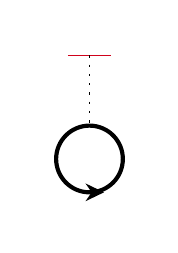
\begin{tikzpicture}[x=0.75pt,y=0.75pt,yscale=-1,xscale=1, baseline=(XXXX.south) ]
\path (0,95);\path (58.66667175292969,0);\draw    ($(current bounding box.center)+(0,0.3em)$) node [anchor=south] (XXXX) {};
%Straight Lines [id:da3194897839790105] 
\draw [color={rgb, 255:red, 208; green, 2; blue, 27 }  ,draw opacity=1 ]   (19.33,13.33) -- (29.78,13.33) ;
%Straight Lines [id:da9155294698759933] 
\draw [color={rgb, 255:red, 208; green, 2; blue, 27 }  ,draw opacity=1 ]   (29.78,13.33) -- (40.23,13.33) ;
%Straight Lines [id:da13142497560962174] 
\draw  [dash pattern={on 0.84pt off 2.51pt}]  (29.78,13.33) -- (29.78,47.19) ;
%Shape: Circle [id:dp8962966421220611] 
\draw  [color={rgb, 255:red, 0; green, 0; blue, 0 }  ,draw opacity=1 ][line width=1.5]  (13.71,63.26) .. controls (13.71,54.38) and (20.9,47.19) .. (29.78,47.19) .. controls (38.66,47.19) and (45.85,54.38) .. (45.85,63.26) .. controls (45.85,72.14) and (38.66,79.33) .. (29.78,79.33) .. controls (20.9,79.33) and (13.71,72.14) .. (13.71,63.26) -- cycle ;
%Straight Lines [id:da7168487847478093] 
\draw [color={rgb, 255:red, 0; green, 0; blue, 0 }  ,draw opacity=1 ]   (29.78,79.33) -- (33.78,79.33) ;
\draw [shift={(36.78,79.33)}, rotate = 180] [fill={rgb, 255:red, 0; green, 0; blue, 0 }  ,fill opacity=1 ][line width=0.08]  [draw opacity=0] (8.93,-4.29) -- (0,0) -- (8.93,4.29) -- (5.93,0) -- cycle    ;
\end{tikzpicture}
+\tikzset{every picture/.style={line width=0.75pt}} %set default line width to 0.75pt        
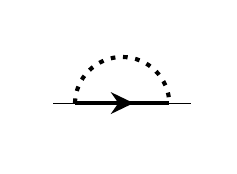
\begin{tikzpicture}[x=0.75pt,y=0.75pt,yscale=-1,xscale=1, baseline=(XXXX.south) ]
\path (0,57);\path (87.33333587646484,0);\draw    ($(current bounding box.center)+(0,0.3em)$) node [anchor=south] (XXXX) {};
%Straight Lines [id:da4779610823231175] 
\draw [color={rgb, 255:red, 0; green, 0; blue, 0 }  ,draw opacity=1 ]   (12.33,36.33) -- (22.78,36.33) ;
%Straight Lines [id:da9873503675232067] 
\draw [color={rgb, 255:red, 0; green, 0; blue, 0 }  ,draw opacity=1 ]   (68.1,36.33) -- (78.55,36.33) ;
%Straight Lines [id:da09313351721820862] 
\draw [color={rgb, 255:red, 0; green, 0; blue, 0 }  ,draw opacity=1 ][line width=1.5]    (22.78,36.33) -- (68.1,36.33) ;
\draw [shift={(51.04,36.33)}, rotate = 180] [fill={rgb, 255:red, 0; green, 0; blue, 0 }  ,fill opacity=1 ][line width=0.08]  [draw opacity=0] (11.07,-5.32) -- (0,0) -- (11.07,5.32) -- (7.35,0) -- cycle    ;
%Shape: Arc [id:dp7767262671888671] 
\draw  [draw opacity=0][dash pattern={on 1.69pt off 2.76pt}][line width=1.5]  (22.78,36.33) .. controls (23.05,23.96) and (33.2,14.05) .. (45.62,14.11) .. controls (58.08,14.17) and (68.16,24.25) .. (68.24,36.67) -- (45.51,36.84) -- cycle ; \draw  [color={rgb, 255:red, 0; green, 0; blue, 0 }  ,draw opacity=1 ][dash pattern={on 1.69pt off 2.76pt}][line width=1.5]  (22.78,36.33) .. controls (23.05,23.96) and (33.2,14.05) .. (45.62,14.11) .. controls (58.08,14.17) and (68.16,24.25) .. (68.24,36.67) ;  
\end{tikzpicture},
\end{equation}
where $W$ is the RPA-screened potential.

\vspace{0.25cm}
\textbf{Why some say $\Sigma(1, 2) = \ii G(1, 2) W(1^+, 2)$?}

\begin{itemize}
    \item $G(1, 2)$ is actually $G(1, 2^+)$ (so when $1=2$, $G = n_{\text{occ}}$: 
    the loop in the Hartree term above)
    \item $\Sigma(1, 2) = \ii G(1, 2^+) W(1, 2) = \ii G(1^-, 2) W(1, 2) = \ii G(1, 2) (1^+, 2)$.
    \item $1^+$ or $2^+$ $\Leftrightarrow$ $\ee^{\pm \ii \omega 0^+}$
        $\Leftrightarrow$ how to take contour 
\end{itemize}

\end{frame}

\begin{frame}
\frametitle{Other tricky details in diagrammatics}

\textbf{Time-reversal symmetry}

\begin{itemize}
    \item $W(- \vb*{p} , -\omega) = W(\vb*{p}, \omega)$ is always true 
        (or otherwise we can symmetrize the Lagrangian)
    \item The real symmetry: 
    \begin{equation}
        \begin{aligned}
            &W(\omega, -\vb*{k}) = W(\omega, \vb*{k}) \Leftrightarrow 
            W(- \omega, \vb*{k}) = W(\omega, \vb*{k})  \\
            \Leftrightarrow &W(\vb*{r}, \vb*{r}', \omega) = W(\vb*{r}', \vb*{r}, \omega) \Leftrightarrow
            W(\vb*{r}, \vb*{r}', \omega) = W(\vb*{r}, \vb*{r}', - \omega).
        \end{aligned}
    \end{equation}
\end{itemize}

\textbf{Imaginary unit} 
\begin{equation}
    \protect\ii G= \ii G_{0} + \ii G_{0} \times 
\underbrace{
    \begin{gathered}
        \tikzset{every picture/.style={line width=0.75pt}} %set default line width to 0.75pt        
        \begin{tikzpicture}[x=0.75pt,y=0.75pt,yscale=-0.6,xscale=0.6, baseline=(XXXX.south) ]
            %\path (0,75);\path (56,0);\draw    ($(current bounding box.center)+(0,0.3em)$) node [anchor=south] (XXXX) {};
            %Shape: Circle [id:dp046942194255674474] 
            \draw  [fill={rgb, 255:red, 155; green, 155; blue, 155 }  ,fill opacity=1 ] (8.54,37.54) .. controls (8.54,27.35) and (16.81,19.08) .. (27,19.08) .. controls (37.19,19.08) and (45.46,27.35) .. (45.46,37.54) .. controls (45.46,47.74) and (37.19,56) .. (27,56) .. controls (16.81,56) and (8.54,47.74) .. (8.54,37.54) -- cycle ;
        \end{tikzpicture}
    \end{gathered}
}_{- \ii \Sigma} \times \ii G
    \Rightarrow G = \frac{1}{\omega - E^0 - \Sigma}.
\end{equation}

\textbf{``Antiparticles''} You can treat holes as antiparticles 
(negative energy, $\ii \sgn(\xi_{n \vb*{k}})$ in time-ordered Green function)
but then corresponding electron modes have to be ignored. 

\end{frame}

\begin{frame}[allowframebreaks]
\frametitle{Feynman rules}

Recall that we are working in a crystal -- we need to talk about $\vb*{G}$ vectors

One set of rules that work: 
\begin{itemize}
    \item Propagator: \begin{equation}
        \begin{gathered}
            \begin{tikzpicture}[x=0.75pt,y=0.75pt,yscale=-1,xscale=1, baseline=(XXXX.south) ]
                \path (0,57);\path (86,0);\draw    ($(current bounding box.center)+(0,0.3em)$) node [anchor=south] (XXXX) {};
                %Straight Lines [id:da8778734653821205] 
                \draw    (5,30) -- (76.5,30) ;
                \draw [shift={(44.55,30)}, rotate = 180] [fill={rgb, 255:red, 0; green, 0; blue, 0 }  ][line width=0.08]  [draw opacity=0] (8.93,-4.29) -- (0,0) -- (8.93,4.29) -- (5.93,0) -- cycle    ;
                % Text Node
                \draw (40.75,23.5) node [anchor=south] [inner sep=0.75pt]    {$n,k$};
                \end{tikzpicture}
        \end{gathered} =
        \frac{\ii}{\omega - \xi_{n\vb*{k}} + \ii 0^+ \sgn(\omega)} \eqqcolon \ii G^0_{n \vb*{k}}(\omega).
    \end{equation}
    \item Interaction: 
    \begin{equation}
        \begin{gathered}
            \begin{tikzpicture}[x=0.75pt,y=0.75pt,yscale=-1,xscale=1, baseline=(XXXX.south) ]
                \path (0,57);\path (86,0);\draw    ($(current bounding box.center)+(0,0.3em)$) node [anchor=south] (XXXX) {};
                %Straight Lines [id:da7824913889732596] 
                \draw  [dash pattern={on 0.84pt off 2.51pt}]  (5,30) -- (76.5,30) ;
                % Text Node
                \draw (40.75,23.5) node [anchor=south] [inner sep=0.75pt]    {$q,\vb*{G}$};
            \end{tikzpicture}
        \end{gathered} =
        - \ii \frac{1}{V} v(\vb*{q} + \vb*{G}).
    \end{equation}
    But the prefactor of the interaction Hamiltonian is still $1/2V$, and 
    \begin{equation}
        v(\vb*{q}) = \int \dd[3]{\vb*{r}} \ee^{- \ii \vb*{q} \cdot \vb*{r}} v(\vb*{r}).
    \end{equation}
    \item For internal lines, 
    sum over $\vb*{k}, n, \vb*{G}$; no additional normalization factors are needed. 
    \item For external lines, 
        outgoing lines are $\phi_{n \vb*{k}}(\vb*{r})$, 
        ingoing lines are $\phi^*_{n \vb*{k}}(\vb*{r})$, as in: 
        \begin{equation}
            G(\vb*{r}, \vb*{r}', \omega) = \sum_{n, \vb*{k}}
            \frac{\phi_{n \vb*{k}}(\vb*{r}) \phi_{n \vb*{k}}(\vb*{r})^*}{\omega - \xi_{n \vb*{k}} 
            + \ii \sgn(\xi_{n \vb*{k}})} ,
        \end{equation}
        where $\vb*{r}$ is the outgoing index and $\vb*{r}'$ is the ingoing index.
\end{itemize}

\end{frame}

\section{$GW$ without $G$}

\begin{frame}
\frametitle{$GW$ without $G$}



\end{frame}

\end{document}